%%%%%%%%%%%%%%%%%%%%%%%%%%%%%%%%%%%%%%%%%
% Kieker Monitoring Component
%
% $Date$
% $Rev$:
% $Author$


\chapter{\KiekerMonitoringPart{} Component}\label{chap:componentsMonitoring}

\NOTIFYBOX{The Java sources of this chapter, as well as a pre-compiled binary, %
can be found in the %
\file{\customComponentsBookstoreApplicationReleaseDirDistro{}/} directory of the %
binary release.}

\section{Monitoring Controller}\label{sec:componentsMonitoring:monitoringController}

\section{Monitoring Records}\label{sec:componentsMonitoring:monitoringRecords}

Monitoring records are objects that contain the monitoring data, as mentioned %
in the previous chapters. Typically, an instance of a monitoring record is %
constructed in a monitoring probe (Section~\ref{sec:monitoring:probe}), %
passed to the monitoring controller (Section~\ref{sec:componentsMonitoring:monitoringController}), %
serialized and deserialized by a monitoring %
writer (Section~\ref{sec:monitoring-log-writers}) and a
monitoring reader, and provided to analysis filters (Section~\ref{sec:analysis:controller}). %
Figure~\ref{fig:KiekerCommunicationDiagram} illustrates this life cycle of a monitoring %
record. %

In Chapter~\ref{chap:example}, we've already introduced and used the monitoring %
record type \class{OperationExecutionRecord}. \Kieker{} allows to use custom %
monitoring record types. Corresponding classes must implement the %
interface \class{IMonitoringRecord} shown in Figure~\ref{sec:monitoringrecord:interfacesAndImplementingClasses}. %
The methods \method{initFromArray}, \method{toArray}, \method{getValueTypes} %
are used for serialization and deserialization of the monitoring data contained %
in the record. Alternatively---in order to support the definition of immutable record types---the %
marker interface \class{IMonitoringRecord.Factory} needs to be implemented, requiring the %
implementation of (i)~the \method{toArray} method (as before), (ii)~a %
constructor accepting a values array, and (iii)~a public static \method{TYPES} %
field. The method \method{setLoggingTimestamp} is used by the monitoring controller to %
store the date and time when a record is received by the controller. %
The method \method{getLoggingTimestamp} can be used during analysis to retrieve %
this value. \KiekerMonitoringPart{} provides the abstract class %
\class{AbstractMonitoringRecord} (Figure~\ref{sec:monitoringrecord:interfacesAndImplementingClasses}) %
which already implements the methods to maintain the logging timestamp.

\begin{figure}[ht]\centering
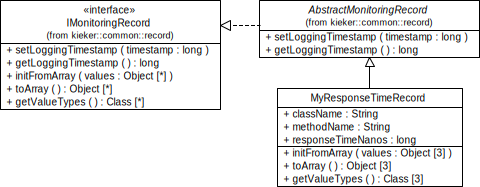
\includegraphics[scale=0.75]{images/kieker_MyRTRecord-modified}
\caption{Class diagram with the \class{IMonitoringRecord} and \class{IMonitoringRecord.Factory} interfaces, the abstract %
class \class{AbstractMonitoringRecord}, and a custom monitoring record type %
\class{MyResponseTimeRecord}}
\label{sec:monitoringrecord:interfacesAndImplementingClasses}
\end{figure}

%  \pagebreak

\noindent In order to use the abstract class for implementing your own monitoring record type, you need to:

\begin{enumerate}
\item Create a class that extends \class{AbstractMonitoringRecord}
\item  and
\begin{enumerate}
\item Override the methods \method{initFromArray}, \method{toArray}, \method{getValueTypes}
\item For immutable record types: implement \class{IMonitoringRecord.Factory}, a constructor %
with a single \class{Object[]} argument, and a public static \method{TYPES} field. %
In this case, \method{initFromArray} (which is not called by the framework then) should %
throw an \class{UnsupportedOperationException}.
\end{enumerate}
\end{enumerate}

\noindent The class \class{MyResponseTimeRecord}, shown in the class diagram in %
Figure~\ref{sec:monitoringrecord:interfacesAndImplementingClasses} and in %
Listing~\ref{listing:MyRecord}, is an example of a custom monitoring record type %
that can be used to monitor response times of method executions. %
Implementing \class{IMonitoringRecord.Factory}, \class{MyResponseTimeRecord} is %
an immutable type, i.e., it includes only final fields. %

\enlargethispage{1cm}

% \pagebreak 

\ % pushing the method initFromArray in the listing to the following page

\setJavaCodeListing
\lstinputlisting[caption=MyResponseTimeRecord.java, label=listing:MyRecord,firstline=27,firstnumber=27]{\customComponentsBookstoreApplicationDir/src/kieker/examples/userguide/ch3and4bookstore/MyResponseTimeRecord.java}

% \pagebreak

\section{Monitoring Probes}\label{sec:monitoring:probe}

The probes are responsible for collecting the monitoring data and passing it %
to the monitoring controller. %
In Chapter~\ref{sec:example:monitoring}, we have already demonstrated how to %
manually instrument a Java application. Listing~\ref{listing:cuttingBookstore} %
shows a similar manual monitoring probe, which uses the monitoring record type %
\class{MyResponseTimeRecord} defined in the previous Section~\ref{sec:componentsMonitoring:monitoringRecords}.

% Make sure that this listing will be modified, once the sourcecode changes!!!
% It must show the whole monitoring of the bookstorecall, from getting the first time to persisting of the record!!
% \pagebreak
\lstinputlisting[firstline=32, lastline=40, firstnumber=32, caption=Excerpt from Bookstore.java, label=listing:cuttingBookstore]{\customComponentsBookstoreApplicationDir/src/kieker/examples/userguide/ch3and4bookstore/Bookstore.java}

\noindent In order to avoid multiple calls to the \method{getInstance} method of the %
\class{MonitoringController} class, singleton instances should be stored %
in a final static variable, as shown in Listing~\ref{listing:cuttingBookstore:finalStaticController}.

\enlargethispage{1cm}

\lstinputlisting[firstline=24, lastline=25, firstnumber=24, caption=Singleton instance of the monitoring controller stored in a final static variable (excerpt from Bookstore.java), label=listing:cuttingBookstore:finalStaticController]{\customComponentsBookstoreApplicationDir/src/kieker/examples/userguide/ch3and4bookstore/Bookstore.java}

\noindent When manually instrumenting an application, the monitoring probe is implemented %
by mixing monitoring logic with business logic, which is often not desired since %
the resulting code is hardly maintainable. %
Many middleware technologies, such as Java~EE Servlet~\cite{JavaServletTechnology-WebSite}, %
Spring~\cite{Spring-WebSite}, and %
Apache~CXF~\cite{CXF-WebSite} provide interception/AOP~\cite{Kiczales1997} interfaces %
which are well-suited to implement monitoring probes. AspectJ~\cite{AspectJ-WebSite} allows to %
instrument Java applications without source code modifications. %
Chapter~\ref{chap:aspectJ} describes the \Kieker{} probes based on these technologies allowing to %
monitor trace information in distributed applications.

\section{Monitoring Writers}\label{sec:monitoring-log-writers}

Monitoring writers serialize monitoring records to the monitoring log/stream and  % and persist the recorded informations into files, databases etc. %
must implement the interface \class{IMonitoringWriter}. The monitoring %
controller passes the received records to the writer by calling the method %
\method{newMonitoringRecord}. Writers can use the methods to serialize the %
record contents, as described in Section~\ref{sec:componentsMonitoring:monitoringRecords}.

% This is the diagram with the hierarchy of the writers.
\begin{figure}[b]%[H]
	\begin{centering}
		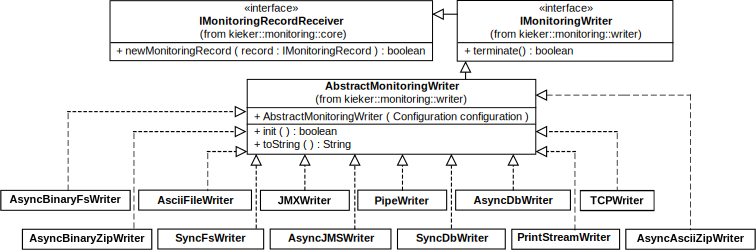
\includegraphics[scale=0.7]{images/kieker_writerimplsuserguide-modified}
		\caption{Interface \class{IMonitoringWriter} and some of the implementing classes}
		\label{figure:monitoringLogWritersHierarchy}
	\end{centering}
\end{figure}

Figure~\ref{figure:monitoringLogWritersHierarchy} shows some fo the monitoring writers %
already implemented in \KiekerMonitoringPart{}. The available properties for the %
included writers are well-documented in the %
example configuration file (see Appendix~\ref{sec:appdx:monitoringproperties}). %

% \enlargethispage{1.2cm}

Different writers can be used %
to store monitoring records to filesystems and databases respectively (e.g., \class{FileWriter}, \class{AsciiFileWriter}, %
\class{SyncFsWriter}, \class{AsyncDbWriter}, and \class{SyncDbWriter}). %
The variants with the prefix \class{Async} are implemented using asynchronous %
threads that decouple the I/O operations from the control flow of the %
instrumented application. %
As the new Kieker writer API uses always a fast pipe implementation to decouple the writer, nowadays all writers are asynchronuous.
Furthermore, the new \class{FileWriter} introduced new features and comes with a standard Kieker text serialization and a binary serialization.
In addition, it can be extended to write other formats.
The \class{AsciiFileWriter} is the default writer that has already been used in %
Section~\ref{sec:example:monitoring}. %
Please note that the database writers are currently in a prototype stage and
that they should be used with care. %
The \class{PrintStreamWriter} simply sends the String representation of incoming %
records to the standard output or standard error streams, which can be helpful %
for debugging purposes.

The \class{JmsWriter} and \class{JmxWriter} write records to a JMS %
(Java Messaging Service~\cite{JMS-WebSite}) queue and JMX (Java Management %
Extensions~\cite{JMX-Website}) queue respectively. The \class{PipeWriter} %
allows to pass records via in-memory record streams (named pipes). %
These writers allow to implement on-the-fly analysis in distributed systems, i.e., analysis while %
continuously receiving new monitoring data from an instrumented application potentially %
running on another machine. A more detailed description of how to use the \class{JmsWriter} %
can be found in Appendix~\ref{appendix:usingJMS}. %

\noindent Listing~\ref{listing:MyWriter} %on page~\pageref{listing:MyWriter} 
shows %
a custom writer \class{MyPipeWriter} which uses a named pipe to %
write the given records into a buffer located in the memory. The source code of %
the class \class{MyPipe} is listed in Appendix~\ref{appendix:pipeListings}. %

\setJavaCodeListing
\lstinputlisting[caption=MyPipeWriter.java, label=listing:MyWriter,firstline=23,firstnumber=23]{\customComponentsBookstoreApplicationDir/src/kieker/examples/userguide/ch3and4bookstore/MyPipeWriter.java}

% \pagebreak

\pagebreak

\noindent The monitoring writer to be used is selected by the %
\KiekerMonitoringPart{} configuration property (Section~\ref{chap:componentsMonitoring}) %
\textit{kieker.monitoring.writer}. Writer-specific configuration properties %
can be provided by properties prefixed by the fully-qualified writer classname.  %
Listing~\ref{lst:monitoringwriter:MyWriter} demonstrates how to use the custom %
writer \class{MyPipeWriter} defined above. In this example, the pipe name is %
passed as the property value \textit{pipeName}.

\setPropertiesListing
\lstinputlisting[caption={Configuration of the custom writer \class{MyPipeWriter}},label=lst:monitoringwriter:MyWriter,firstline=5,firstnumber=5,lastline=6]%
{\customComponentsBookstoreApplicationDir/src-resources/META-INF/kieker.monitoring.properties}

\enlargethispage{1cm}

\noindent As the data structure of this kind of monitoring stream, we created a %
class \class{PipeData} in order to demonstrate the use of the \method{toArray} and %
\method{initFromArray} (in Section~\ref{sec:analysis:reader}) methods. %
A \class{PipeData} object holds a logging timestamp and an \class{Object} array %
containing the serialized record data. %
Appendix~\ref{appendix:pipeListings} includes a source code listing of this class. %
Alternatively, we could have used \class{IMonitoringRecord} as the data structure %
used by the pipe. This is the way, \Kieker{}'s \class{PipeWriter} works. %
